\documentclass[11pt, titlepage]{article}
\usepackage{amsmath,amsthm,amssymb}
\usepackage{hyperref, pgf, tikz}
\usepackage{fancyhdr}
\usetikzlibrary{arrows}
\usepackage[margin=1.25in]{geometry}
\usepackage{graphicx}                     
\pagestyle{fancy}
\usepackage{array}
\usepackage{indentfirst}
%\usepackage{wrapfig}

\lhead{Lab \#6}
\rhead{\thepage}
\cfoot{}

\title{Introduction to the Microwave Optics System and Reflection \\ \ \\ \large Lab \#6}
\author{Name: Avery Karlin \\ Partner: Dalton Wu}
\date{}
\begin{document}

\maketitle

\begin{center}
\LARGE Introduction to the Microwave Optics System and Reflection
\end{center}

\section*{Objective}
The objective of the lab is to practice using the microwave optics system, measure the relationship between distance and microwave strength, and test the law of reflection.

\section*{Introduction}
Electromagnetic radiation is perpendicular transverse waves of magnetic and electric fields, all moving at the speed of light ($3 * 10^8$ m/s), ranging in type based on frequency and energy, with higher frequency meaning higher energy. The most high energy is gamma radiation, produced by nuclear reactions only, unlike all other forms which are produced by electronic movement. The next longest is x-rays, used in medical testing, followed by ultraviolet, then visible light (the only type humans can see), followed by infrared (used for night vision, based on black body radiation), then microwave radiation, and finally radio waves (used for all electronic communication signals).

Electromagnetic radiation can be polarized by a polarizer, only allowing waves of a specific orientation through, such that perpendicular polarizers block all waves as a result. Microwave strength is inversely proportional to the square of the distance, such that it decreases exponentially. In addition, the law of reflection states that if the radiation is reflected, the angle of incidence is equal to the angle of reflection, such that the microwave radiation picked up is greatest at that angle from it.

\section*{Procedures and Results}

First, 

\begin{figure}[h]
\centering
\hspace*{0cm}
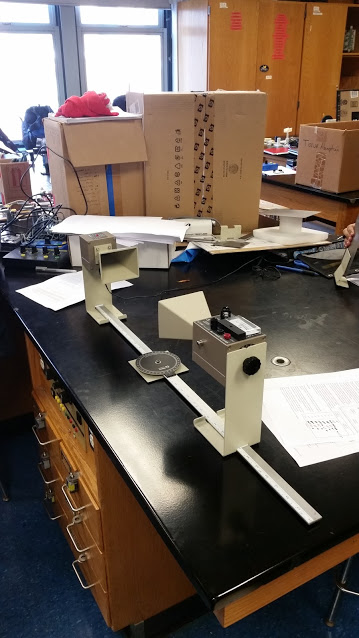
\includegraphics[scale=1]{lab61.jpg}
\vspace*{0cm}
\end{figure}

\begin{figure}[h]
\centering
\hspace*{0cm}
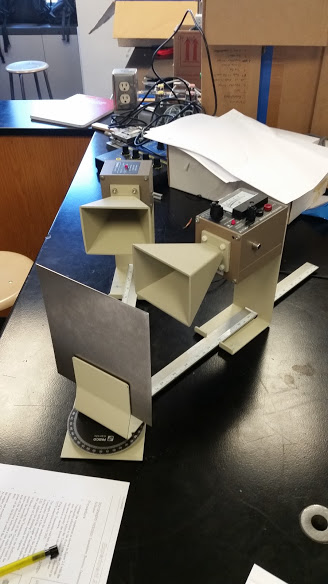
\includegraphics[scale=1]{lab62.jpg}
\vspace*{0cm}
\end{figure}

\underline{Wave Strength vs Distance:}
\begin{center}
\begin{tabular}
{|m{9em}|m{12em}|}
\hline
Distance (m) & Microwave Radiation Strength (M) \\
\hline
0.4 & \\
\hline
0.5 & \\
\hline
0.6 & \\
\hline
0.7 & \\
\hline
0.8 & \\
\hline
0.9 & \\
\hline
1 & \\
\hline
\end{tabular}
\end{center}

\underline{Wave Strength vs Distance:}
\begin{center}
\begin{tabular}
{|m{9em}|m{12em}|}
\hline
Distance (m) & Microwave Radiation Strength (M) \\
\hline
0.4 & \\
\hline
0.5 & \\
\hline
0.6 & \\
\hline
0.7 & \\
\hline
0.8 & \\
\hline
0.9 & \\
\hline
1 & \\
\hline
\end{tabular}
\end{center}

\underline{Wave Strength vs Distance:}
\begin{center}
\begin{tabular}
{|m{9em}|m{12em}|}
\hline
Distance (m) & Microwave Radiation Strength (M) \\
\hline
0.4 & \\
\hline
0.5 & \\
\hline
0.6 & \\
\hline
0.7 & \\
\hline
0.8 & \\
\hline
0.9 & \\
\hline
1 & \\
\hline
\end{tabular}
\end{center}

\section*{Discussion}
Sample calculations for the non-measured data are as shown using the formulas found above:

$$RC_{exp} \text{(Trial 1, Resistance)} = \text{Divisions per 0.63 rise} * \text{Sweep Time per Div} = 2.1 * 2 = 4.2 ms$$
$$RC_{calc} \text{(Trial 1, Resistance)} = R * C = 10k \Omega * 1 nF = 10 ms$$
$$\text{Percent Error (Trial 1, Resistance)} = \frac{\text{$|$Expected - Actual$|$} * 100\%}{\text{Expected}} = \frac{|4.2 - 10| * 100\%}{10} = 58\%$$

\underline{Wave Strength vs Distance:}
\begin{center}
\begin{tabular}
{|m{9em}|m{12em}|}
\hline
Microwave Radiation Strength$^2 (M^2)$ & \\
\hline
0.4 & \\
\hline
0.5 & \\
\hline
0.6 & \\
\hline
0.7 & \\
\hline
0.8 & \\
\hline
0.9 & \\
\hline
1 & \\
\hline
\end{tabular}
\end{center}

For the change in resistance, the main error seems to be that resistance doesn't impact the time constant experimentally. This is due to the resistance being affected by the frequency, such that the change in resistance for the same frequency has to be far greater to impact the experimental time constant. As a result, for the same frequency and capacitance, within a small region of changes in the resistance, the time constant is the same experimentally for RC circuits. In addition, difficulty operating the oscilloscope itself can account for a portion of the error. In addition, additional resistance due to non ideal wires could bring the experimental time constant up relative to the actual time constant to some degree, though this appears to have had a generally minor effect. 

\section*{Conclusion}

The time constant for the resistance changing trials, for a calculated RC of 10 ms was 4.2 ms with 58\% error, 5 ms was 4.2 ms with 16 \% error, and 3 ms was 4.2 ms with 40\% error. Thus, the slope of $\tau$ vs R was 0 F to the actual capacitance of 1 nF for a percent error of 100\%. The time constant for the capacitance changing trials, for a calculated RC of 7 ms was 5.4 ms with 22.9\% error, and 4 ms was 2.4 ms with 40\% error. Thus, the slope of $\tau$ vs C was 3 $k\Omega$ to the actual resistance of 10 $k\Omega$ for a percent error of 70\%.

\end{document}
